\begin{comment}
1. Introdução
    - Aprendizado Supervisionado
    - Aprendizado Não Supervisionado 

2 - Fundamentação

3. Trabalhos relacionados 
    - Métodos/algoritmos
4. Metodologia
    3 PAGINAS

\end{comment}

\chapter{Fundamentação Teórica}\label{cap:fundamentacaoteorica}

Neste capítulo serão apresentados alguns métodos importantes para o entendimento do trabalho. Tais métodos têm como objetivo,  a criação de atributos numéricos a partir de um conjunto de palavras (documentos). Alguns métodos destinam-se à criação de atributos como, \textit{Bag-of-words} apresentado na Seção  \ref{sec:bag-of-words} e \textit{N-gram} na Seção \ref{sec:ngram}. Outros métodos como \textit{TfIdf}, Seção \ref{sec:tfidf} e Stemização Seção \ref{sec:stem} tem como objetivo a atribuição de valores às características do documento.


\section{\textit{Bag-of-Words}}\label{sec:bag-of-words}
Um modelo \textit{bag-of-words}, ou BoW, é uma maneira de extrair atributos do texto para alimentar os algoritmos de aprendizado de máquina. Na abordagem, olha-se para o histograma das palavras dentro do texto, ou seja, considerando cada contagem de palavras como uma característica \cite{goldberg2017neural}. 

\textit{Bag-of-words} é uma representação de texto que descreve a ocorrência de palavras em um documento. Como pode ser visto na Figura \ref{fig:exemplo-bow}, as palavras dos documentos são separadas de forma distinta montando vetores que representam {\it palavra} e {\it frequência}, na qual {\it palavra} é o termo usado no documento e a {\it frequência} é o número de vezes que esse termo aparece nos documentos.

Qualquer informação sobre a ordem ou estrutura das palavras no documento é desconsiderada. O modelo só se preocupa com o fato de palavras conhecidas ocorrerem no documento e não com sua localização.

\begin{figure}[ht]
  \centering
  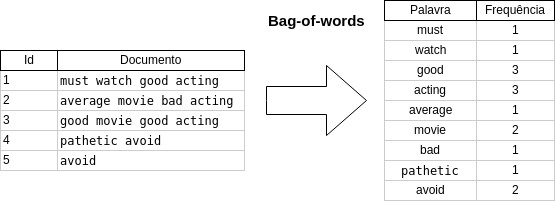
\includegraphics[height=0.2\textheight]{figuras/exemplos/bow-exemplo.png}
  \caption{Exemplo do uso de BoW.}
  \label{fig:exemplo-bow}
\end{figure}

\section{{\it N-gram}}\label{sec:ngram}
N-gramas de textos são amplamente utilizados em tarefas de mineração de texto e processamento de linguagem natural.  N-gram são basicamente uma sequência de termos com o comprimento de $N$ caracteres. 

Usando como exemplo a Figura \ref{fig:exemplo-ngram}, ao utilizar N-gram em um determinado documento, cada termo é dividido em $N$ sequências. Tendo $N=1$ (unigram) cada termo é separado individualmente. Para o $N=2$ (bigram), os termos são divididos de dois em dois e o mesmo serve para o $N=3$. Cada termo criado pelo \textit{N-gram} pode ser representado como uma nova característica, como mostra na Tabela \ref{tab:exemplo-ngram}.  

\begin{figure}[ht]
  \centering
  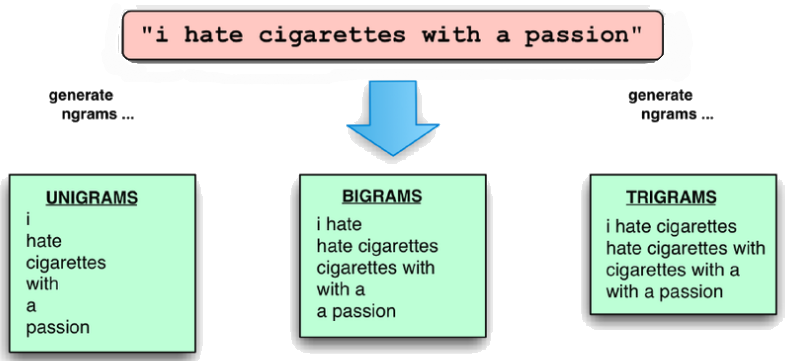
\includegraphics[height=0.3\textheight]{figuras/exemplos/ngram-exemplo.png}
  \caption{Exemplo do uso de N-gram. \cite{exemplongram}}
  \label{fig:exemplo-ngram}
\end{figure}


\begin{table}[h]
\scalebox{0.8}{
\begin{tabular}{c|c|c|c|c|c|c|c|c}
\hline
 {\bf Documento} & \textbf{a} & \textbf{a passion} & \textbf{cigarretes} & 
 \textbf{cigarretes with} & \textbf{cigarretes with a} & 
 \textbf{hate} & \textbf{hate cigarretes} & \textbf{...} \\
 \hline
\textbf{1} & 1 & 1 & 1 & 1 & 1 & 1 & 1 & ... \\
\textbf{2} & 0 & 0 & 1 & 1 & 0 & 0 & 0 & ... \\
\textbf{3} & 1 & 1 & 0 & 0 & 0 & 0 & 0 & ... \\ \hline
\end{tabular}
}
\caption{Exemplo de características utilizando N-gram.}\label{tab:exemplo-ngram}
\end{table}


\section{TF-IDF}\label{sec:tfidf}
O \textit{TF-IDF} tem como objetivo atribuir um peso para as palavras que aparecem com menos frequência nos documentos. Muitas vezes a importância de uma palavra não se dá somente pela sua frequência. 

Documentos maiores, geralmente, são representados por muitos termos. Quando uma grande quantidade de termos é utilizada na representação de documentos, a probabilidade do termo pertencer a um documento é alta e, assim, documentos maiores têm melhores chances de serem relevantes do que documentos menores \cite{tfidf-martins2003metodologia}, como é o caso de \textit{bag-of-words}, visto na Seção \ref{sec:bag-of-words}.

O \textit{term frequency (tf)} é uma métrica que utiliza o número de ocorrências do termo $tj$ no documento $di$. No entanto, quando termos com alta frequência aparecem em todos (ou na maioria) dos documentos da coleção, os mesmos não fornecem informação útil para os atributos nos documentos. Assim, a medida \textit{inverse document frequency (idf)} favorece termos que aparecem em poucos documentos da coleção. As definição do TF e do IDF serão apresentadas a seguir:

\[ tf = \frac{tj}{di} \]
onde $tf$ é o número de vezes que o termo $tj$ ocorre no documento $di$.

\[ idf = log(\frac{d}{t}) \]
onde $t$ é o número de documentos que contém o termo e $d$ é o número total de documentos (\textit{corpus});

\[ tfidf = tf * idf\]
no qual as medidas $tf$ e $idf$ são combinadas.

\section{Stemização}\label{sec:stem}
Na criação da tabela atributo-valor utilizada por algoritmos de Aprendizado de Máquina, cada termo que aparece no documento pode ser mapeado como uma coluna na tabela. Assim, o número de dimensões do conjunto de atributos pode ser grande, gerando  um problema que deve ser minimizado. 

Vários métodos podem ser utilizados a fim de reduzir a quantidade de atributos visando uma melhor representatividade e melhor desempenho do processo de predição. Entre outros, a transformação de cada termo para o radical que o originou, por meio de algoritmos de stemização (\textit{stemming}), é um método amplamente utilizado e difundido, conforme \cite{tfidf-martins2003metodologia}.

Segundo \cite{jivani2011comparative}, a stemização é uma etapa de pré-processamento na mineração de textos e recuperação de informação,  bem como um requisito muito comum de funções de processamento de linguagem natural (PNL). Podemos dizer que o objetivo da stemização é reduzir palavras para uma forma mais básica e comum de escrita. A ideia principal é melhorar o manuseio automático de terminações de palavras, reduzindo as mesmas às suas raízes de palavras. Geralmente, a stemização é feita removendo quaisquer sufixos e prefixos (afixos) anexados nas palavras, dado que o radical de um termo representa um conceito mais amplo do que o termo original. Na Tabela \ref{tab:exemplo-stem} é exemplificada a aplicação da stemização para a redução das variações do radical \textit{quilometr}.

Na stemização, a conversão de formas morfológicas de uma palavra ao seu tronco é feita supondo que cada um é semanticamente relacionado. O radical não precisa ser uma palavra existente no conjunto de atributo-valor, mas todas as suas variantes devem ser mapeadas para este radical. Há dois pontos a serem considerados ao usar o método de stemização:

\begin{itemize}
    \item se as formas morfológicas de uma palavra têm o mesmo significado básico, devem ser mapeadas para o mesmo radical;

    \item palavras que não têm o mesmo significado devem ser mantidas separadamente.
\end{itemize}

Essas duas regras são boas o suficiente, desde que os valores resultantes sejam úteis para a mineração de texto ou PNL. Segundo \cite{jivani2011comparative}, a utilização da stemização é geralmente considerada como um dispositivo de melhoria de revocação (frequência em que um classificador encontra os exemplos de uma classe). Para linguagens com morfologia relativamente simples, a influência da stemização é menor do que para aquelas com morfologia mais complexa.

% exemplo stemização
\begin{table}[h]
    \centering
    % distancia entre a linha e o texto
    {\renewcommand \arraystretch{1.25}
        \begin{tabular}{ l | l }
            \hline  
            \textbf{Palavra} & \textbf{Stem} \\  
            \hline
            quilométricas & quilometr \\  
            quilométricos & quilometr \\  
            quilômetro & quilometr \\  
            quilômetros & quilometr \\  
            \hline
        \end{tabular} 
    }
    \caption{Exemplo de Stemização}\label{tab:exemplo-stem}
\end{table}

Um dos algoritmos de stemização mais conhecidos é o algoritmo de Porter que remove sufixos de termos em inglês \cite{porter2001snowball}.

\section{KNN}\label{sec:knn}
O KNN ({\it K-Nearest-Neighbor}, em português, K-vizinho mais próximo) é um classificador que procura K documentos do conjunto de treinamento que estejam mais próximos deste documento com classificação desconhecida, ou seja, que tenham a menor distância.

Estes $K$ documentos são chamados de K-vizinhos mais próximos. Verifica-se quais são as classes desses K vizinhos e a classe mais frequente será atribuída à classe do documento desconhecido.

\begin{figure}[ht]
  \centering
  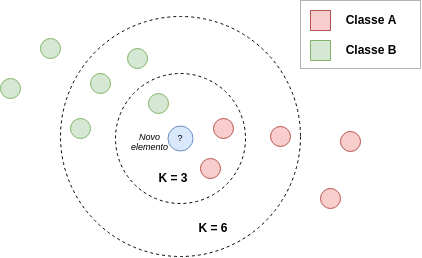
\includegraphics[height=0.2\textheight]{figuras/exemplos/exemplo-knn.png}
  \caption{Exemplo de execução do KNN.}
  \label{fig:exemplo-knn}
\end{figure}

Como pode ser observado no exemplo da Figura \ref{fig:exemplo-knn} a classificação de um novo elemento (em azul) para o $K=3$. Todos os vizinhos mais próximos desse novo elemento são classificados com a classe $A$, portanto, o novo elemento será classificado com a classe $A$. Para o $K=6$, a maioria dos vizinhos mais próximos são de classe $B$, então o novo elemento é classificado como sendo de classe $B$.

A métrica mais comum que calcula a distância é a distância Euclidiana \cite{santos2009variaccoes}. Seja $X=(x_1, x_2,..., x_n)$ e $Y=(y_1, y_2,..., y_n)$ dois pontos de $R^n$, a distância Euclidiana entre X e Y é dada por: 
\[d(x, y) = \sqrt{(x_1-y_1)^2+(x_2-y_2)^2+...+(x_n-y_n)^2}\]
